%\documentclass[conference]{usenix}
%\documentclass[conference]{IEEEtran}
%\documentclass[twocolumn,8pt]{article}
%\usepackage{times}
\documentclass[letterpaper,twocolumn,10pt]{article}
\usepackage{usenix,epsfig,endnotes}
\usepackage{mathptmx}
\usepackage{epsfig,color}
\usepackage{cite,url}
\usepackage{amsmath}
%\usepackage{mdwlist}


%\addtolength\columnsep{0.5em}

%\parindent=0em

\newcommand{\XXX}[1]{\textbf{\small [XXX: #1]}}
\newcommand{\JNX}[1]{\textbf{\small [XXX: #1 --JN]}}

\newcommand{\uexp}{_\mathrm{exp}}
\newcommand{\umax}{_\mathrm{max}}
\newcommand{\ceil}[1]{\left\lceil#1\right\rceil}

%\renewcommand\baselinestretch{0.92}%\footnotesize\normalsize
\newcommand{\car}[1]{\left|#1\right|}

\makeatletter
  \newcommand\tabcaption{\def\@captype{table}\caption}
\makeatother

%\pagestyle{empty}
\begin{document}


%\title{Groups: A generic security architecture for networked systems}
\title{S-Groups: Reusable security components for networked systems}
\if 0
\author{
{\rm Atul Singh}\\
Rice University
\and
{\rm Lakshminarayan Subramanyam}\\
Intel Research Berkeley
\and
{\rm Petros Maniatis}\\
Intel Research Berkeley 
\and
{\rm Timothy Roscoe}\\
Intel Research Berkeley
\and 
{\rm Peter Druschel}\\
Max Planck Institute for Software Systems 
}
\fi
\maketitle


\abstract{
Blah..
}

\section{Motivation}
Typically, security is an afterthought in design and construction of large scale systems. Designers first build a distributed system and reason about its properties: correctness, scalability, overhead and ease of use etc. Once it is understood and ready to be deployed in the wild, the designers start to worry about the possible vulnerabilities and come up with mechanisms to defend the system. Morever, the techniques proposed in the literature to defend against possible malicious attacks are targeted toward a specific attack~\cite{}. They are effective against the attack they defend against, however these defenses are not generic and the effectiveness of mechanisms is not based on thereotical foundations such as BFT~\cite{}. Finally, as newer systems are being designed and implemented, newer techniques for defending against malicious behavior are being investigated and developed (e.g., fork consistency~\cite{}). It is not yet clear if is there a systematic way of applying the plethora of security work on rapidly-emerging large scale systems, which would definitely ease up the deployment of newer systems in the wild.


To bridge this gap between innovative techniques for fault-tolerance and their application to wide range of large-scale systems, we propose the \textit{group} abstraction as a first class design principle for constructing such large scale systems. Intuitively, it allows us to break the complexity and functionality of such large scale systems in smaller pieces, which not only allows us to understand and reason about the system more coherently but enables us to implement suitable mechanisms (either security oreinted or system oriented) at groups. Our work has the following two high level themes:
\begin{itemize}
\item{} We articulate the usefulness of group abstraction when thinking about such large scale systems. Existing systems implicitly build groups but do not bring up this abstraction as a design principle.
\item{} Allows us to employ well-understood fault-tolerance techniques at the group abstraction and extract gaurantees (security related or others) from groups.
\end{itemize}

To show the usefulness of the group abstraction, we first model the secure routing technique~\cite{} using group abstraction and show how group abstraction helps us not only to reason about the technique and apply it to other systems but also to improve its performance. Next, we use our group abstraction to improve the fault-tolerance of Credence~\cite{}, a widely-popular object reputation system. Finally, we apply our group abstraction to PRACTI, a replication framework.

\section{Groups in existing systems}
Some existing systems use group structure for handling certain operations, e.g. replica groups in DHT's provide load-balance and fault-tolerance. However, the usage of group structure is rather ad-hoc and it is not clear if there is any resemblance between group structure used in one system and another.
We can informally divide existing large scale systems in three classes: (a) no notion of groups, (b) implicit groups and (c) explicit groups.

\paragraph{No Groups:} PRACTI.

\paragraph{Implicit Groups:} DHT's like Pastry/Chord which define leafsets and routing table's and these are sort of groups.

\paragraph{Explicit Groups:} CoralCDN uses explicit groups (called \textit{clusters} in their terminology) for improving the latency and load-balance.


\section{Our vision}
We envision that an application designer will re-factor his/her application using groups and then configure the groups according to the requirements. Figure~\ref{fig:thin-waist} shows the architecture for builiding group-based large scale systems. The configuration interface is divided into three parts: communication, computation and management.


\begin{figure} 
\begin{center} 
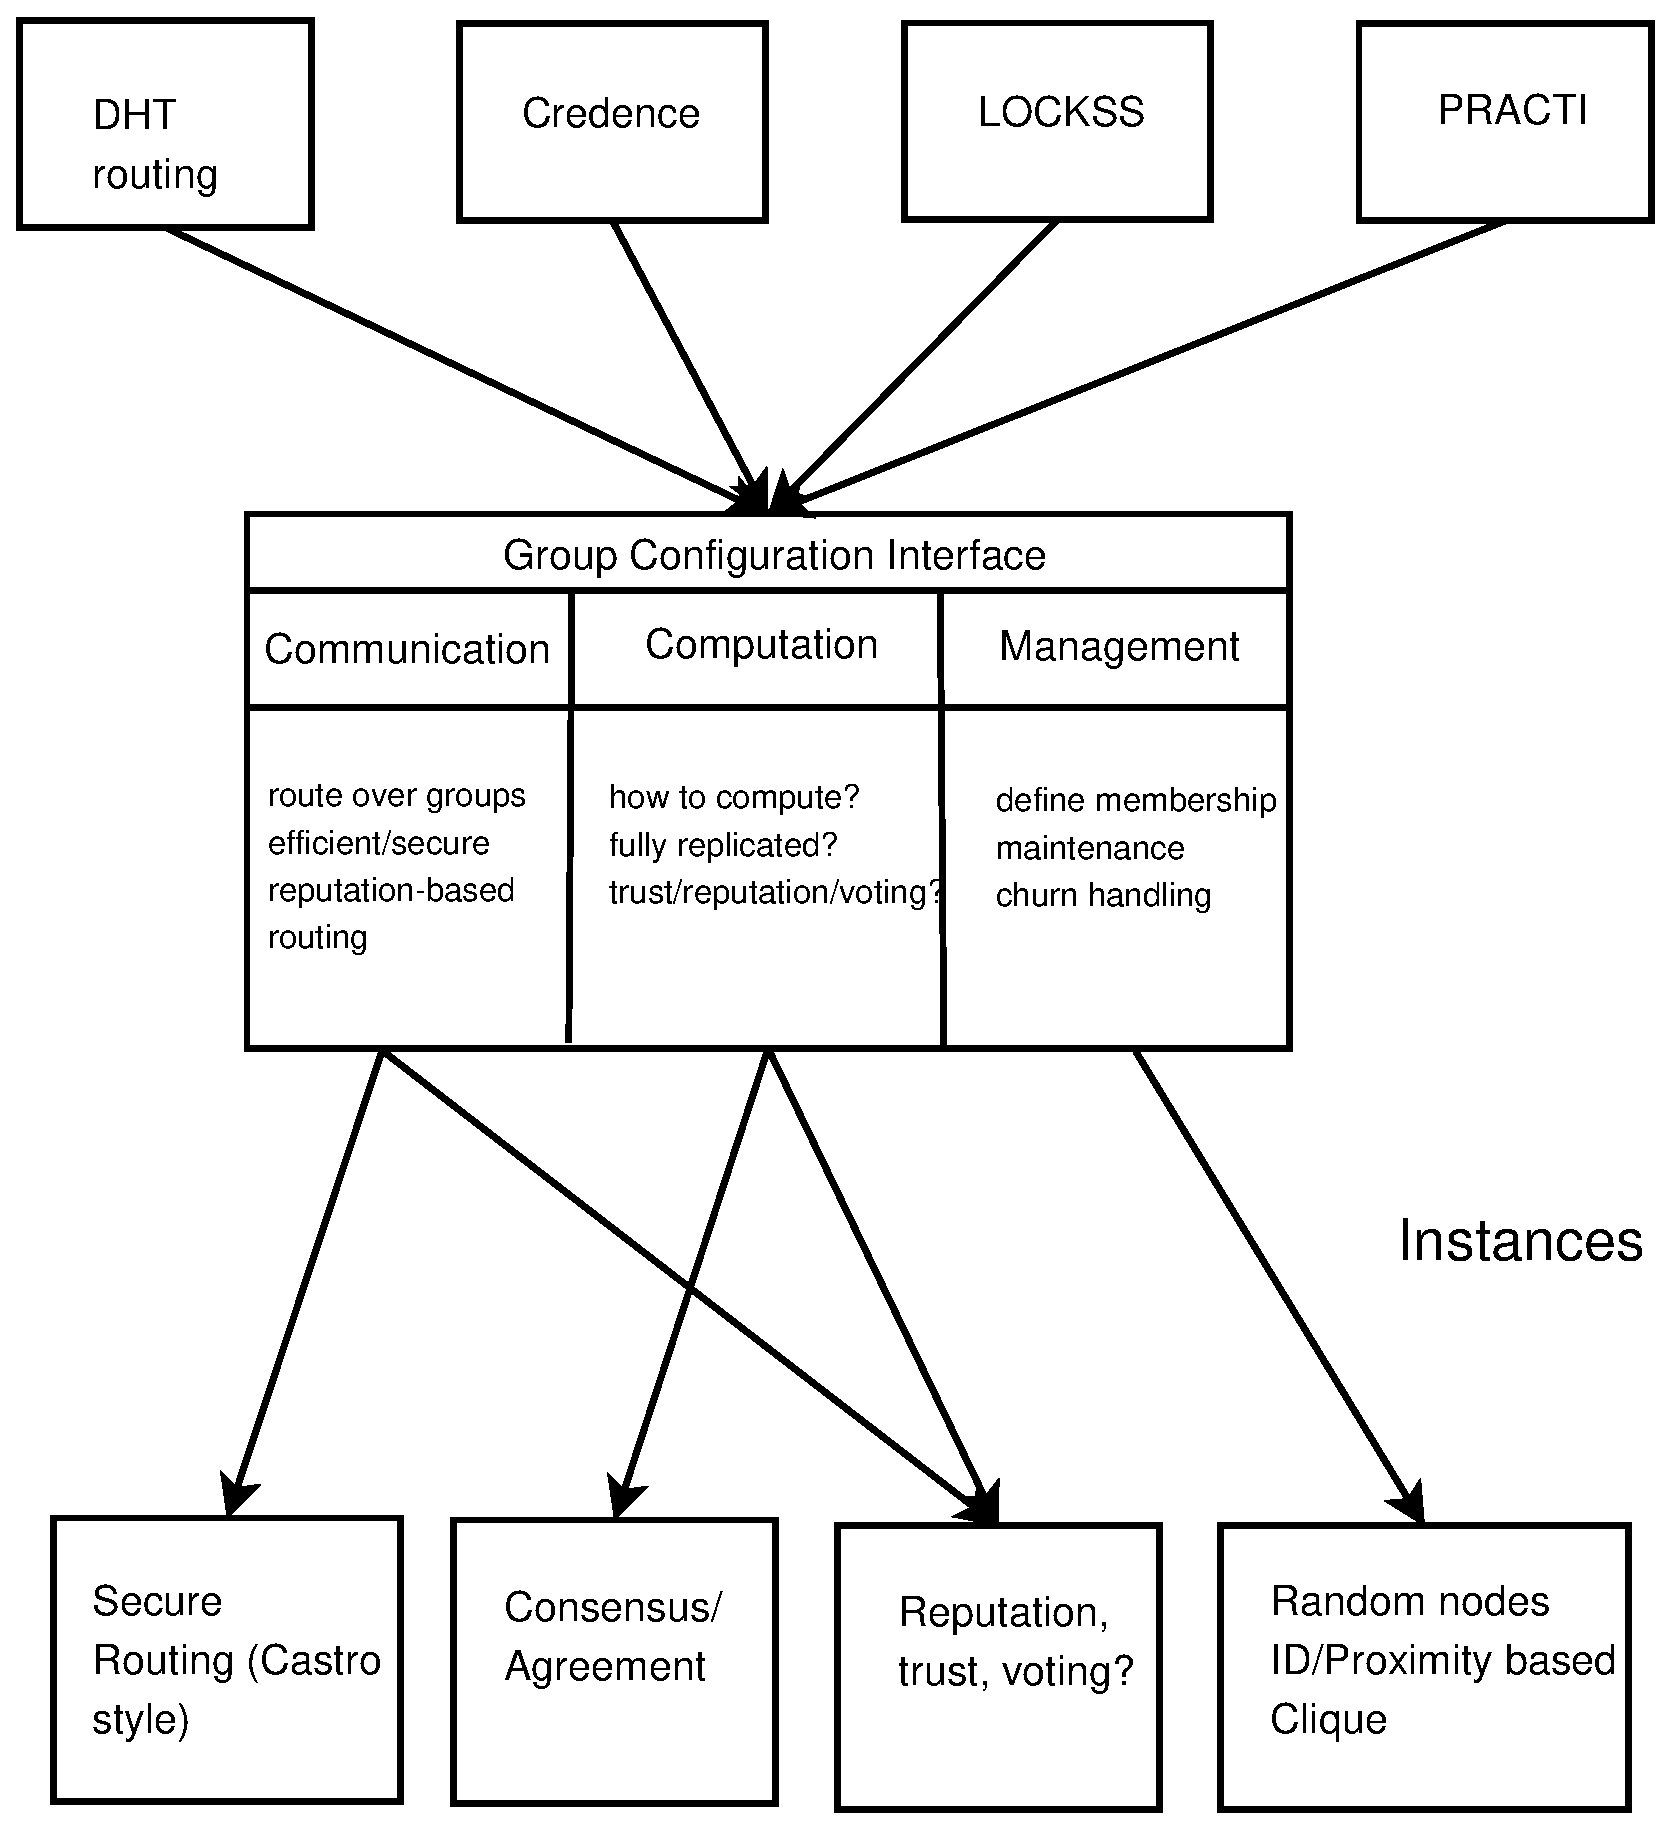
\includegraphics[width=3in]{thin-waist.eps} 
\end{center} 
\caption{Architecture}
\label{fig:thin-waist} 
\end{figure}

\paragraph{Management Interface:} It is used to define the group members (size), how are they selected (random), how is the group maintained (as a clique) and how do we handle dynamism (periodic heartbeats). Note that the way groups are defined affects the resilience of each group.

\paragraph{Communication Interface:} This defines two aspects: routing state and how forwarding is done. Application designer specifies how routing state is maintained and how is routing done (secure routing ala Castro style redundant routing or reputation based routing).

\paragraph{Computation/Service Interface:} This allows the designer to specify the service and the way group version of the service is implemented. For example, in a DHT, a \texttt{get()} operation may be based on voting of every member of the group storing that object.


\section{Example 1: G-DHT's}
DHT's provide two basic functionality, \texttt{put()} and \texttt{get()}, similar to a centralized hashtable. Moreover, these two functionalities are preceded by \texttt{lookup()} operation which involves multi-hop routing. We now show how would G-DHT (Group-DHT) work.

\paragraph{Joining the G-DHT}
Joining the G-DHT overlay implies joining the group associated with a node. This operation follows the join operation suggested in the literature for DHTs: ask a bootstrap node to route to your group. Routing proceeds over groups (whether secure or efficient is configurable) and message ultimately reaches your group. After that, you inform your group members and thereby join the group. Group maintenance and membership functions need to be configurable.

\paragraph{Routing in G-DHT}
A group consist of set of nodes and therefore routing over groups can be implemented in many fashions, e.g. one-to-one, one-to-all, many-to-one or many-to-many. This brings up the tradeoff between overhead and fault-tolerance. Castro's secure routing primitive uses one-to-one routing and hopes that at least one path is malicious free so that it reaches one correct node of the destination group.

\paragraph{Operation 1: \texttt{put()}}
After correct group is reached, \texttt{put()} operation can is performed over the group. For fault-tolerance, this operation can be performed over the whole group or a subset of the group. 

\paragraph{Operation 2: \texttt{get()}}
After correct group is reached for an object, \texttt{get()} operation can be either performed over a single node of a group or a subset of the group or the whole group. For self-certifying data, it is easier to check the correctness of data and hence one can perform this operation optimistically at one node. For mutable data, it may be important to get an agreement over the most-recent version of the data and hence one may need to execute this operation over sufficient number of group members. So, given an operation, we might need agreement functionality from the groups.

\paragraph{Cost} Certain optimizations may not be possible. For example, perfect PNS may not be possible.

\paragraph{Lessons learned}
We need interface for following operations:\\
1. Group membership \\
2. Group maintenance \\
3. Communication \\
4. Computation or service provided\\
Note that 3 and 4th point show that any networked system has two building blocks: communication and computation. Both needs to be made reliable, with possibly different techniques.

\section{Example 2: G-Credence}
Credence is based on Gnutella, so it shares the vulnerabilities associated with unstructured overlays. Credence introduces two new functionalities, vote gather and gossip. Both are vulnerable to malicious tamper. Again, it relies on lookup operation to find an object which is typically implemented as constrained flood. We assume for now that overlay join and normal lookup is done similarly to G-DHT.

\paragraph{Vote gather in G-Credence}
Nodes ask other nodes to vote on an object. Based on the trust placed on that node, its vote is weighted. Malicious nodes can vote arbitrarily on objects. A vote by a group on an object is simply a majority of the votes given by the group members. So, a misbehavior of a single node does not affect the decision taken by the correct node. This assumes that sufficient number of group members are correct.

\paragraph{Gossip in G-Credence}
Credence relies on random gossip to find nodes and their votes on different objects. However, this random gossip is favored toward nodes with good trust value. Instead, if trust value is based on group of nodes, then gossip is more fault-tolerant (assuming again that sufficient group members are good).

\paragraph{Cost} Behavior of each node counts toward the trust value of the whole group.So, each group member might need to fetch the object and rate it themselves before responding to other groups. 


\section{Challenges}
What are the main challenges in making such an abstraction practical?

\begin{itemize}
\item{} define group abstraction
\item{} work assignment problem
\item{} handle dynamism inside the groups as well as at group level
\item{} develop appropriate versions of existing fault-tolerance approaches (probabilistic approach, weak consistency) for low overhead 
\item{} define an interface so as to be usable to designers 
\item{} Example applications
\end{itemize}

\subsection{Metrics to define groups}
\paragraph{Membership: flexible or strict}
A basic question is what identifies a group? Since we are targetting security and fault-tolerance, one metric is that the membership function should be verifiable. For example, suppose nodes who share first $k$ bits in their ids form a group. Here, node's id automatically defines its membership in a group. If node's id is its IP address, then one way to define a group could be the node's who share the network address, then IP address automatically defines the group membership. The above two examples satisfy our verifiability property if ids are secure and ip address is not spoofed.
Note that there are other choices of defining a group: node's within $\delta$ delay from each other form a group (as in CoralCDN), friends within $k$ hop from each other in a social network etc. Since these metrics are hard to verify by a third-party, they do not satisfy our verifiability metric.

\paragraph{Overlapping or non-overlapping groups}
What is the benefit of having overlapping groups?


\paragraph{Size of groups: uniform or non-uniform}

\paragraph{Number of groups: variable or fixed} .

\subsection{Work assignment problem}
Now, once group membership is defined, we need to partition the workload among different groups. Note that the workload is application dependent and potentially the partitioning algorithm too. As an example, the lookup queries in DHTs form its workload and workload partitioning is done automatically based on their identifiers. By exposing the group abstraction, we provide greater flexibility in the hands of the designer in selecting appropriate work assignment among groups. For example, rather than choosing the closest group to a query, one can replicate the work to multiple groups.

Note that we again require this work division process to be verifiable so as to identify if a node in a group is not providing the service it is supposed to.

\subsection{Extracting gaurantees from groups}
Assume for a moment that the group as a whole follows the specification correctly. With this assumption, each group can be now thought of as a correct state machine and the whole system as a collection of such correctly behaving individual state machines. Our goal is to provide such abstraction of correctly behaving groups out of possibly malicious individual group members and thereby relieving the system designer of providing security mechanisms for every system he designs.

Since our goal is to provide security properties which are general and have theoretical base, we have couple of choices to choose from the well studied approaches to fault-tolerance:
\begin{itemize}
\item{BFT:} This requires that the group should have at least $3f+1$ members if it can have at most $f$ byzantine faulty nodes.
\item{Byzantine Quorum Systems:}  This requires that the group should have $5f+1$ members if it needs to tolerate $f$ byzantine faulty nodes. This is more scalable than the BFT approach in terms of throughput, however it needs more servers. Moreover, each client access a subgroup (a quorum) and the requirement is that the subgroups intersect in at least $2f+1$ members to ensure consistency.
\end{itemize}

Straight-forward application of these techniques to large scale systems is problematic due to:
\begin{itemize}
\item{} at large scale, some groups will inevidently have more than $f$ byzantine faults and the whole groups functionality might be compromised. A possible solution is to increase the group size such that with very high probability, each group has sufficient number of correct nodes. However, the overhead of BFT technique scales up with increasing size, which is bad. Not sure about BQS.
\item{} These techniques assume the client-server model, and these requirements are essentially on the servers. A key observation is that in large scale p2p systems, there is no such explicit distinction: each node is a server for some workload and a client for some other workload. Can we leverage such symmetric communication to provide better results?
\item{} Detecting misbehaving group member and cancelling its membership is not considered in these techniques and the reasons is that failure detection in asynchronous networks is not accurate~\cite{}. However, if we relax the synchrony assumptions, what kind of failures can we detect? 
\end{itemize}


Failure detection techniques typically used:
\begin{enumerate}
\item{Auditing:}
\item{Secure history entanglement:}
\item{Voting:}
\item{BFI:}
\item{Fork-consistency:}
\end{enumerate}

\paragraph{Node failure detection} 


\paragraph{Group failure detection}


\subsection{Handle dynamism}
We need to consider dynamics at two levels: group level and node level. 

more on this later..

\if 0
\section{Interface}
There are two ways to go about interface issue. (a) The algorithm is modified so that the basic entity used is a group and interface translates group functionality to individual node functionality. (b) The algorithm is unmodified (uses individual nodes) and we provide the interface for translation from node to group behavior. We first focus on the first approach (its not clear yet which one is more useful).


\subsection{Group to node translation (Type-I)}
Translating group functionality to node functionality involves defining two parts: group membership and graph structure. Our goal is to ensure that the graph structure at group level imposed by the application is achievable through the graph to node translation. Note that the first part can be independent of the application.

First, we enumerate the functionality needed for group membership and maintenance:
\begin{enumerate}
\item{group definition:} How do we define groups? This is an abstract definition.
\item{group join:} How does a node joins a group G?
\item{group leave:} When do we say that a node has left group G?
\item{group members:} Given a group, how do we identify its group members? Is there a primary member of a group?
\item{group maintenance:} How does individual nodes maintain the group?
\end{enumerate}

Now, we enumerate the functionality needed for providing application oriented graph structure:
\begin{enumerate}
\item{inter-group links:} what links does a node has to maintain in order to map it to the links at the group level as specified in the algorithm? In other words, how does graph strcture at group level transform to graph structure at node level?
\item{routing:} how does routing proceed at node level to correspond to routing at group level?
%\item{intra group routing:} Given a message to the group, how is it routed to the destination node in the group? If there is a primary, it should be delivered to it.
%\item{inter group routing:} Given a message, how does a message is routed to a destination group?
\end{enumerate}

The exact interface looks like as follows:\\
\texttt{
1. void defineGroup(size k, PolicyGroupDef p)\\
2. Group join(NodeId nid) \\
3. void leave(NodeId nid, GroupId G) \\
4. boolean isMember(GroupId gid) \\
5. Group members(GroupId gid) \\
6. void groupMaintenance(PolicyGroupMaintenance p)\\
7. void defineLink(GroupId G1, GroupId G2, PolicyEdge p, int power) \\
8. void linkMaintenance(PolicyEdgeMaint pem) \\
9. Group route(Message M, PolicyRouting rp, SecGaurantee g, PNSReq p)\\
}

\subsection{Node to group translation (Type-II)}
later...

\section{Pastry using Group Abstraction (Type-I)}
Lets assume for now the constrained version of Pastry routing table.
Assumption: we assume a defense against Sybil attack and a certified authority to provide random identifiers to nodes with associated public-private key pairs.

First, we explain the high order idea of group membership. Each node forms a group with its own id. Other nodes are k/2 nodes on the left and k/2 nodes on the right. So, each node is a member of k groups. In each group it is member of, it knows all the members. 

Now, the high order idea for graph structure. Pastry specifies a way of maintaing routing table such that prefix routing can occur. Each node's routing table slot now points to a group rather than a node. Depending on the configuration, the group mapping for each routing slot could be done by either keeping one node from that group or multiple nodes from that group. For constrained routing table, we keep one entry whose id is closest to the id of the slot. For proximity aware routing, we keep one entry which is closest among the group responsible for that slot. If you want, you can proceed directly to Section~\ref{sec:gaurantees_pastry}. Next two subsection provide the details on how to implement this.

\subsection{Group membership}


\paragraph{\texttt{defineGroup}:} Groups in Pastry are specified by PolicyConsecutiveId, which implies that given the nodeid of a node, group is the set of k+1 nodes: k/2 on the left and k/2 on the right of nodeid (id's are consecutive). This means that each node is a member of $k$ groups and the identifier of a group is the id of the middle member. Given a key $K$, the group who is responsible for it is the group whose id is closest to $K$. Note that this definition of group is slightly different from the leafsets in Pastry as nodes in Pastry do not maintain the full information for all the groups. Also, groups are overlapping in this example, two consecutive groups overlap in $k$ nodes.

%\paragraph{\texttt{join}:} The join request of the new node is routed to the group who is responsible for its node id. The group members are returned in the response. New node finds out the potential members of its own group abouts its existence. This causes the members of its group members to join the new group (by calling \texttt{joinGroup()}) and also make them leave another group (by calling \texttt{leaveGroup()}).

\paragraph{\texttt{isMember()}:} A node needs to check for which groups it is part of. For Pastry, it is easier to calculate this check. Given a group id, it can check the various groups it is part of. This method returns true if the group id to check for lies between the leftmost and rightmost groups it is part of. Otherwise, it returns false. Note that this is closely related to the PolicyConsecutiveId.

\paragraph{\texttt{members()}:} When one group communicates to other group, we need to define how nodes communicate on behalf of groups. In Pastry, this function returns the $k/2$'th entry from the group members when they are sorted. For secure versions, we might need to return the full member set.

\paragraph{\texttt{join}:} A node needs to join a new group when a newer group is formed or an earlier group is dissolved. All this happens tranparently to the application. For the groups specified for Pastry, a node will have to leave a group when a node leaves or a new node joins. The logic to calculate membership is defined earlier. A node needs to join a group when one of the groups it is member of leaves the overlay. The algorithm is simply to check on what side of groups the dead group lies and find the next group in that direction and join it.

\paragraph{\texttt{leave()}:} This also happens tranparently to the application. A group leave happens when a new node arrives in the system and a node has to join the new group and leave an existing group. A leave also happens when a node leaves the overlay.

\paragraph{\texttt{maintenance}:} Group maintenance is specified by the \texttt{PolicyGroupMaintenance}. For Pastry, it means periodically talking to every member of the group.

%Nodes in a group periodically talk to each other. This helps in identifying any failed nodes. Since accurate failure detection is not possible, we need probabilistic failure detection. We denote a node as failed if more than $f$ nodes in the group observe it to have failed in a given time period. Note that this dependence on synchrony does not make us vulnerable to attacks since when a node is marked failed, another member automatically joins the group. Since each node is malicious with some probability, malicious nodes can only increase the overhead.
\subsection{Graph structure and routing}
Pastry specifies a unique way of arranging links between different groups to obtain a specific graph structure. Additionally, it specifies a way of routing over the links (prefix based routing). 


\paragraph{\texttt{defineLink}:} The \texttt{EdgePolicy} spcifies what edges to form from group G1. For Pastry, the policy specifies the following logic:\\
it maintains a link between $G_1$ and $G_2$ if
\begin{equation}
0 \le x \le 128/b, 0 \le y \le 2^b, G_2 = id(G_1, x, y)
\end{equation}
where $id(G,x,y)$ represents an id whose x'th digit is y and remaining are similar to G and $b$ is the number of bits in each digit. Any node who is a member of group $G_1$ will first route to the destination $G_2$ and obtain the full member set. Now, there are couple of choices here. It might keep the full set for greater security, or pick the one which is closest in proximity. Each choice gives different properties. Power of a link specifies exactly how many nodes it keeps for each group to group link.

\paragraph{\texttt{linkMaintenance}:} This is specified by \texttt{PolicyEdgeMaintenance}. For Pastry, it amounts to pinging the node pointed to by the edge periodically, but at a frequency lower than the group maintenance.

%\paragraph{Routing state} Each node needs to maintain some amount of routing state to allow it to contact the members of different groups it is part of. Similarly, each group in turn needs to maintain some routing state to contact the other groups. This boils down to the fact that each node needs to maintain two levels of routing state: one for intra-group communication and other for inter-group communication. For Pastry, the routing state for intra-group communication boils down to maintaing live connections with each member of the group. For inter group routing state, each node maintains connection to one member of the group defined by the slot of its routing table. Slot(i,j) of a node n with nodeid id is defined as the identifier whose first i digits are similar to the id and jth digit is j and remaining are similar to id. The group identified by the slot(i,j) is the group whose identifier is closet to this id. Note that with this definition of slot(i,j), the group member pointed by all the groups of a node themselves form another group. In all, each node maintains log(N) connections, achieving connectiosn to log(N) other groups.

\paragraph{\texttt{route()}:} Now routing at node level is exactly similar to routing at group level. Depending on the \texttt{members()} function, either a primary node is returned to the application or the full member set. Note that routing finishes in $O(log(N))$ hops.

\subsection{Extracting properties from groups}
\label{sec:gaurantees_pastry}
By defining the different flavors of \texttt{defineLink} and \texttt{route}, we show how we can provide latency properties as well as security properties from groups.

\subsubsection{Proximity routing}
If \texttt{defineLink()} interface is configured with power set to 1 and PolicyLink specifying the closest node (in terms of proximity) among the members being chosen, then we achieve a variant of proximity neighbor selection (PNS). Interestingly, Gummadi et al~\cite{routing_geometry_sigcomm_03} showed that choosing the closest node from set of $n$ consecutive nodes gives us almost all the benefit of PNS routing when we could choose from very large set (typically $n=16$). However, this version of proximity aware neighbor selection is different from vanilla Pastry but potentially similar gains.
%An additional benefit of this approach is that the underlying group structure is maintained which allows us to reason about the security properties while at the same time improve the latency performance. 


\subsubsection{Secure routing}
Secure routing requires two builiding blocks: secure neighbor selection and secure forwarding.

If \texttt{defineLink()} interface is configured with power set to 1 and PolicyLink specifying the primary node for the group being chosen, then we acheive the constrained version of Pastry routing table. This enables secure neighbor selection.

Castro et al. suggest a mechanism for secure forwarding. It can be divided into two stages: discovery and confirmation. Discovery phases attempts to reach the leafset of the destination key. Confirmation phase attempts to identify every member of the leafset. The probability of successful routing is dependent only on discovery phase and we focus on that here.

Discovery phase is implemented by routing redundantly toward the destination. A node who starts redundant routing first forwards the message to its own group members. Each of the group members pick a next hop node and forward. A key observation is that these set of next hop nodes in fact form a group in our definition. So, routing is actually happening at group level. Again, if secure neighbor selection is enabled and these neighbors are used for forwarding, we achieve the same probability of success as reported by Castro et al. [no?]

 This mechanism works on the assumption that there exists a malicious free path from the origin group to the destination group. This is more constraining than is necessary to achieve secure discovery. In fact, as long as overhead is not a concern, one can flood each group and still discover the destination group as long as each group has at least one correct node. By appropriately configuring the \texttt{defineLink()} and \texttt{route()} interfaces, one can achieve different setting of overhead and security gaurantees. Figure~\ref{fig:redundant-routing} shows the bits.

\begin{figure} 
\begin{center} 
\includegraphics[width=3in]{redundant-routing.eps} 
\end{center} 
\caption{Original redundant routing and its variants which are made possible by defining the inter-group communication pattern. The red node represent the malicious nodes. Note that (c) is obtained by super-imposing (a) and (b).} 
\label{fig:redundant-routing} 
\end{figure} 


\section{Overlay Multicast}

\section{Coral CDN}
CoralCDN uses Kademlia overlay for arranging nodes in the ring and uses XOR routing metric. 

\subsection{Groups for Kademlia}
Kademlia uses bit-XOR between two nodes as the distance between them and maintains 160 routing entries. The $i$'th routing slot contains $k$ nodes who are between $2^i$ to $2^{i+1}$ distance from the local node. 

Let a group be a set of $l$ consecutive id's. Observe now that $i$'th routing slot of these $l$ consecutive nodes are also consecutive (when nodes are uniformally distributed around the ring). So, the node-level graph structure imposed by Kademlia protocol easily maps to the group-level graph structure with our definition of groups.

\subsection{Additional Structure imposed by CoralCDN}
Nodes maintain routing table as suggested by Kademlia. However, CoralCDN places additional structure for content-placement to enable efficient (fast) retrieval. It introduces a notion of cluster (group in our terminology) which is based on following definition:
\begin{itemize}
\item{Locality based groups:} Each node in the group is at most $\delta$ ms away from threshold fraction of group members. $\delta$ is different for different \textit{levels} of groups. For example, level 0 groups have $\delta=20$ while level 1 groups have $\delta=60$ms. 
\item{Non-overlapping:} Groups at level 0 are non-overlapping. Each node decides for itself which group it would join. It may even start a new group if it is not close enough to any group at level 0.
\item{Non-uniform sized groups:} There is no explicit bound on the size of groups and due to variable delay distribution, groups may be of variable sizes. Across levels, groups will be of different sizes with high expectation.
\end{itemize}
\fi
\section{Credence: Object reputation system}

\subsection{How does it work?}
Reputation is for the objects rather than for the peers. Additionally, honest nodes will have similar reputation for a given object. 

Voting to aggregate how other nodes rate a given object. Weighted aggregation to give more weights on honest nodes.

Incorporates transitive reputation for finding out rating of objects not seen by local neighbors.

Attack model: malicious nodes introduce decoys and provide them when asked. No other malicious behavior considered. Assumes a very tiny fraction of malicious participants. Also, the authors explicitly say that we need other techniques to defend against arbitrary attacks. Our goal is to see if our group abstraction can provide exactly that.

\subsection{Vulnerabilities of Credence}
What would happen if there are proactive attacks by the adversary. Moroever, what fraction of malicious entities can it handle for correct results?

Now, we illustrate the vulnerabilities that Credence has when a proactive adversary is involved:
\begin{enumerate}
\item{Overlay structure:} Malicious nodes mounting attack on overlay structure can cripple Credence since the only nodes it is able to communicate might be malicious nodes. Moreover, it has been shown that malicious nodes need not be very large in number for such unstructured overlays.
\item{History-based trust calculation:} A malicious node could remain in the system for long time and build a good reputation with a correct node. By compromising sufficient neighbors of a given node, one could affect the decision taken by a good node. Moroever, a malicious node may have inconsistent behavior with different nodes and this inconsistency may not be discovered.
\item{Colluding adversaries:} What would happen if there are colluding adversaries in the system? If a malicious node has its colluding nodes as its immediate neighbors, auditing them would not help in detecting whether it is mounting an attack. Basically, they can provide arbitrary correlation values for its colluding neighbors.
\end{enumerate}

\subsection{Improving Credence}
Credence already requires nodes to have public/private key pair and a nodeid from a CA to contain the impact of Sybil attacks. We form the group structure as the groups formed for securing the Patry. However, that is not sufficient to defend against all the above attacks. 


\paragraph{Secure trust calculation:} Credence uses the correlation between voting history to evaluate the trust between two nodes to use as weight during the voting calculation. A malicious node who behaves correctly for some time to gain good trust with a good node may corrupt the credibility of future objects. Moreover, if sufficient number of malicious nodes are ranked higher in terms of trust, they can screw up the voting caculation and cause good nodes to reject good objects. This requires us to prevent a node from providing arbitrary vote to a given object and also prevent a malicious node to bias the search for gossiping the vote database. 

This means that biasing the search for votes based on the past correlation can be tailored toward malicious nodes. This is problematic. A mix of random and trust must be used if we want this search to be robust. This defines how inter-group routing works (secure version will go through multiple nodes of a group).

\paragraph{Defense against inconsistent behavior:} Malicious node may provide conflicting rankings for a same object to confuse good nodes. Moroever, this type of behavior may not be noticeable if correct nodes blindly accept their votes. If the group abstraction provides a facility of rendezevous for other nodes to contact and access the history of votes casted by a group member, then this vulnerability can be fixed. Here, a malicious node has to commit to its votes and these votes are independent of who is asking. Malicious nodes now can not tailor its response based on who is asking.Groups provide secure history of the voting cast by the group members.

\paragraph{Defense against collusion:} A set of colluding malicious nodes who are neighbors of each other can prevent a good node from correctly auditing their behavior. This is because a malicious node could choose its neighbors. This behavior can be potentially prevented by forcing a node to commit its behavior to its neighbors where its neighbors are random members of the system. This is obtained by providing random nodes as the group members. Again, the basic group structure of our overlay routing provide a random subset of system as group members.

\paragraph{Stronger gaurantees:} Now, given these defenses, can we obtain more gaurantees from the group abstraction. For example, can we identify the malicious node who supplies decoys? Basically, can we add accountability as a feature to our group abstraction? If a node gives a bad vote to an object, we may want to know the reason. Or if a node provides a good vote to a decoy, we want to know the reason.


\subsection{Overhead of group abstraction}
Note that the overlay members of Gnutella are random members and there is no correlation between the interests of a node and its overlay members. So, changing the overlay members from random nodes to nodes with specific identifiers does not affect the overhead, though it changes the structure of the overlay. The additional overhead of maintaining secure history (of votes casted by nodes) of group members can be potentially reduced by piggy-backing such information on group membership messages. Finally, the overhead of auditing depends on how frequently we do auditing. 

\section{SUNDR}

\section{LOCKSS}

\section{PRACTI}
PRACTI is a replication framework which simultaneously provides partial replication (PR), arbitrary consistency (AC) and topology independence (TI). Earlier systems provide two of the three properties. This enables PRACTI to provide better tradeoffs and provides a single architecture which subsumes most of the design space for development of newer replication systems.

It is based on following four principles:
\begin{itemize}
\item{Log exchange:} BAYOU style
\item{Separate body from control of invalidations:}
\item{Partial invalidations:}
\item{Separation of policy from mechanisms:}
\end{itemize}

Fault-tolerance (both benign and byzantine) is not considered in PRACTI and therefore it is an ideal candidate for our group abstraction approach to fault-tolerance. We assume for now that client write's are authentic, i.e. a server can not forge a client's write operations. We focus on the server corruption.

To handle arbitrary behavior of servers, we use our group abstraction. Nodes in a given group can either form BFT agreement for each read and write operation.

So, following components need to be made fault-tolerant:
\begin{itemize}
\item{Secure log exchange:} When servers exchange their logs, we need to prevent servers from holding certain invalidations. The exchange protocol may involve exchange of control or body of invalidations, or imprecise invalidations.
\item{Secure invalidation propagation:} A server should propagate invalidation messages to nodes who have subscribed to the objects.
\end{itemize}

What do we want from our groups?\\
1. agreement on write order\\
2. propagation of invalidations to other groups \\
3. secure log exchange between groups \\

\paragraph{Agreement on write order}
We want to ensure that members of a group agree on a write order. PRACTI/BAYOU rely on Lamport clocks to ensure that different writes are totally ordered. However, malicious nodes can play with their lamport clocks and prevent replica's from agreeing on the correct write order. One solution is to have BFT style agreement phase, where a write is issued to the primary of a group who serializes the different writes. 

\paragraph{Propagation of invalidations}

\paragraph{Secure log exchange}

\if 0
\section{Detailed secure routing example}

Castro et al. proposed secure routing primitive to handle malicious behavior in p2p routing framework. The basic algorithm is following:
\begin{enumerate} 
\item{} route using the routing table and get the resulting leafset 
\item{} do a density check, if fails go to 3 else return success with the leafset 
\item{} do redundant routing 
\end{enumerate} 
 
Redundant routing works as follows: 
\begin{enumerate} 
\item{} redirect the message through the local node's leafset 
\item{} each node forwards the message according to its routing table 
\item{} if destination key is in the leafset of local node, respond to the originator 
\item{} originator collects the set of nodes who responded, call it tentative set 
\item{} originator send a confirmation request to each member in the tentative set, asking it to verify if the nodes in the tentative set are in fact its view of leafset 
\item{} each such node checks if tentative set is its leafset, if not,  forwards the original message to remaining nodes in its leafset; responds with confirmation  
\item{} repeat step 5 through 7 at most 4 times 
\item{} tentative set is the result 
\end{enumerate} 
 
The probability of successfully reaching the correct leafset with redundant routing is 0.9999 for leafset size of 16. 
 
\subsection{Groups in p2p routing} 
Now, let us formulate the secure routing primitive in terms of groups. Here we assume the constrained version of Pastry routing table, which is similar to Chord routing table. 
 
Let a group $G_{ID}$ is a set of $k$ nodes whose identifiers are closest to ID.  
The leafset of a node forms its primary group. Each node is a member of $k$ groups. Total number of groups in a system of size $N$ is $N$. 
 
Each node maintains connections to $O(log(N))$ groups. Each such connection is maintained via a connection through a group member of that group. Each slot of the pastry routing table points to a group, rather than a node. Essentially, each slot is a set whose size can be made configurable. The entries in the routing table slot $(i,j)$ of the primary group of a node $A$ forms a primary group of another node $B$ whose ID is closest to $ID_{i:A(D-i)}$ (meaning the first i digits are i and remaining are the suffix of ID of A of length D-i).  
 
So, at a group level, group $A$ (which is a primary group of node $A$) maintains neighboring links with $O(log(N))$ other groups. 
 
\begin{figure} 
\begin{center} 
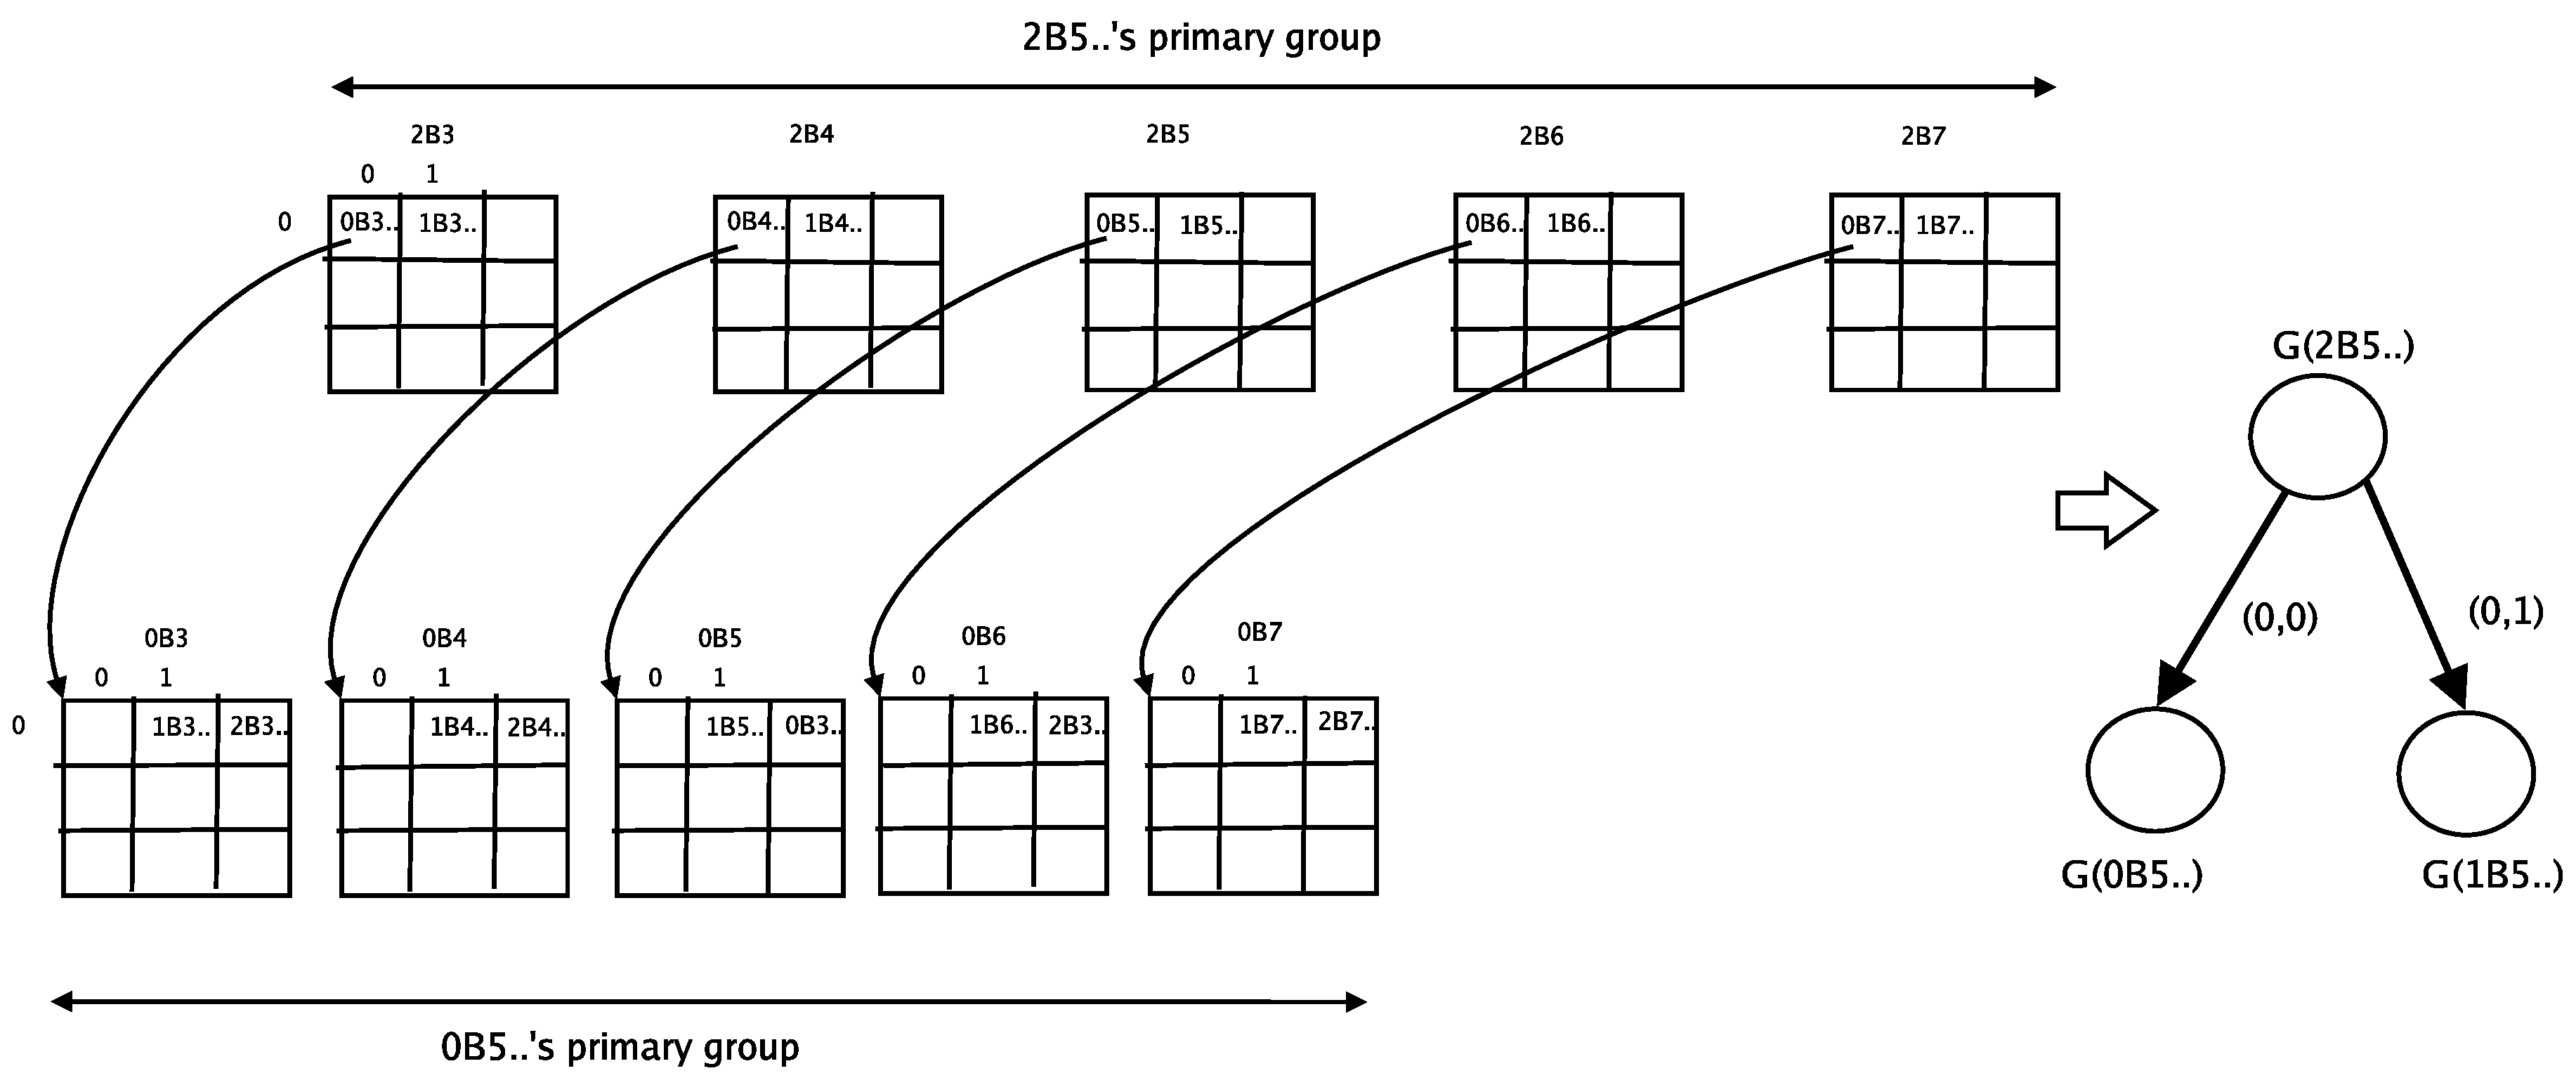
\includegraphics[width=3in]{group-routing-table.eps} 
\end{center} 
\caption{Routing table at node level and at the group level} 
\label{group-routing-table} 
\end{figure} 
 
 
Figure~\ref{group-routing-table} shows the relevant bits. 
 
Prefix-based routing occuring at node links can be viewed as routing happening at group level links. Let the routing start at group $G_{A}$ and key be $K$. First hop of routing reaches a group $G_{K(1):A(D-1)}$, similarly $i$'th hop reaches a group $G_{K(i):A(D-i)}$.  
 
\subsection{Secure routing using groups} 
Assume $A$ is routing for key $K$. 
Version of basic routing: 
\begin{enumerate} 
\item{} send to the first hop group $G_{K(1):A(D-1)}$ and get the resulting group 
\item{} verify group correctness (using density check or other means), if yes, return else  
\item{} do redundant routing 
\end{enumerate} 
 
Now, we can translate the redundant routing in terms of routing at group level: 
\begin{enumerate} 
\item{} send to our primary group 
\item{} route the message to next hop group 
\item{} if local node belongs to the primaryGroup(K) respond to the origin group 
\item{} collect the tentative group and ask that group to confirm the tentative group directly 
\item{} when a node recieves the confirmation, it checks whether other group members are there, if not it forwards to its remaining members and confirms 
\item{} repeat 4 through 5 at most 4 times 
\item{} tentative group is the result 
\end{enumerate} 
 
\begin{figure} 
\begin{center} 
\includegraphics[width=3in]{redundant-routing.eps} 
\end{center} 
\caption{Original redundant routing and its variants which are made possible by defining the inter-group communication pattern. The red node represent the malicious nodes. Note that (c) is obtained by super-imposing (a) and (b).} 
\label{redundant-routing} 
\end{figure} 
 
Figure~\ref{redundant-routing} shows how the original redundant routing works and different variants of redundant routing which are made possible by defining the inter-group communication. 
 
 
It is clear that if each node maintains a single entry in its routing table for its neighboring groups links, then the probability of success is similar to what is achieved by original redundant routing. However, we can do better than that. Rather than forwarding through the single entry in its routing table, if nodes in a group gossip about their entries during intra-group communication, each node has more information about their neighboring groups.  

 
\subsection{Content distribution networks: CoralCDN} 
 CoralCDN consist of three components: set of DNS nameservers, set of http proxies and origin server nodes. DNS nameservers are responsible for redirecting the lookups from unmodified browsers to appropriate http proxies. HTTP proxies are responsible for handling the http requests and finding the requested content at appropriate coral nodes. Coral nodes consist of origin content servers which may be low capacity end hosts providing content. Goal of Coral is to distributed the content providing load across the network such that the overhead on the origin servers is minimized, even under flash crowd effects.

Coral organizes nodes in multiple levels (3 currently) based on their network latency. Nodes in level 2 cluster (group in our terminology) are within 20ms delay to each other. Nodes in level 1 are 60ms delay to each other while every node is a member of level 0 cluster. Lookups first go to level 2 cluster to provide better latency, and then traverse other clusters. Insertions are sloppy in nature, meaning that an insertion may not reach the closest node to the key but stop at either a \textit{full} or \textit{loaded} node. This prevents overloading the nodes closest to a popular key.

\subsubsection{Group abstraction for CoralCDN}
The group definition is the same as cluster definition in Coral: set of nodes who are within 20ms of each other become part of a group at level 2. Each node is a member of one group at each level. However, groups at different levels will interleave (nodes within 20ms of each other will be part of a group at level 2 and also at level 1 and level 0). Nodes within 50 ms will be part of a group at level 1 as well as level 2.

\paragraph{Group joining}
In benign settings, joining a group is exactly how it is defined in the CoralCDN.

\paragraph{Lookup}
Lookup operations proceed first at the intra-group level and if content is not found, inter-group forwarding happens. Lookup now proceeds as the search at the intra-group level before moving on to the next group.

\paragraph{Insertion}

\paragraph{Extracting gaurantees}
 
\subsection{Caching system: Beehive} 
 
 
\subsection{Reputation system: Credence} 
 
\subsection{Anonymization: Cashmere}

\subsection{Sensor networks}

\fi

\section{How to implement it?} 
Is P2 a right system to implement this functionality? 
 
\section{Related work to read} 
1. abstract regions for sensor networks (Matt welsh, NSDI)\\ 
2. ISIS (Birman)\\ 
3. Fault-tolerant gossip\\ 
4. Astrolabe (Cornell) \\ 
5. ISIS: process group approach for building reliable distributed systems (Birman)\\ 
\paragraph{Group Spreading (John-Hopkins)}
Survivability: no single node is eclipsed by malicious nodes

Assumptions: loosely synchronized clocks, bound on message delays between correct nodes

Motivation: random node ids is not sufficient as malicious nodes could remain in the system for a long time and deteriorate the randomness

Idea: enforce a bound on lifetime, generate random identifiers each time and each peer maintains O(log(N)) virtual nodes. each node maintains links to logarithmic sized regions rather than a single finger/link. routing proceeds in groups.

problems: this is basically secure routing of castro but with tolerating a form of sybil behavior.additionally, its not clear to me how they prevent malicious nodes from compromising a group..


\if 0 
\section{Motivation} 
Large scale systems need to tolerate faults, be they benign faults or byzantine faults. Most of the proposed systems either do not provide any fault-tolerance gaurantees or if they do, they are custom made for the system and require analysis of their own. In this project, we seek to apply the traditional and well studied techniques of Byzantine Fault tolerance algorithms (either quorum based or agreement based) to such large scale applications.  
 
\section{Byzantine Fault Tolerance} 
 
\subsection{Quorum-based} 
Malki and Reiter et al. style algorithms 
 
Quorum Systems~\cite{} divide the set of servers into set of subsets (quorums) and use one quorum for read while another quorum for write operations with the assumption that at there is at least one common server between any pair of quorums. However, this is a weak assumption can break the consistency property (read might return a stale value) if the common server between read and write server is malicious. To handle $b$ Byzantine faults, $b$-masking Byzantine Quoram systems~\cite{} have been proposed which assume that between any two quorums, at least $2b+1$ are common. To improve efficiency, probabilistic Byzantine Quorum systems have been proposed~\cite{} which ensure the consistency property with a high probability and work under the assumption that the number of correct nodes among any pair of quorums is greater than the number of bad nodes in any given quorum. 
 
Properties of quorum systems: as $f$ increases, the size of quorums increase. However, since there is no server-to-server communication involved, the server overhead remains fixed as quorum size increases. However, the overhead on clients increases. 
 
However, directly applying these techniques in large scale distributed systems is problematic due to three main reasons: first, these techniques do not handle dynamism in the set of servers and in the quorums; secondly, they assume a fixed set of bad servers in each quorum. First problem is much easier to understand since such large systems typically exhibit fair amount of dynamism. Enforcing a bound on each quorum even when the bound on bad entities in full system is enforced depends on the selection of quorums. For example, if leaf set members of Pastry~\cite{} are chosen as quorum members, then even if $f$ fraction of nodes in the system are malicious, in any given quorum, more than $f$ fraction could be malicious. In fact, the fraction of  malicious nodes will follow some probabilistic pattern. We need to motivate also with a non-p2p application. Third problem is that these techniques do not scale to large systems, where number of participants range to thousands of servers. Finally, these approaches distinguish between the client and server behavior which may not hold for large scale systems. 
 
\subsection{Agreement based} 
 
Castro and Liskov style algorithms 
 
\section{Our Goal} 
 
We intend to extend the probabilistic Byzantine Quorum systems for large scale distributed systems by handling the above two problems. Also, we exploit certain charactersitics of large scale distributed systems to improve the efficiency of our protocols.  
 
Concretely, our goals include: 
\begin{itemize} 
\item{Handle dynamism} 
\item{Handle large scale} 
\item{Exploit probabilistic $f$ in each quorum} Of course, this depends on how quorums are selected. 
\item{Relaxed gaurantees}  
\item{Keeping fast path fast}  
\end{itemize} 
 
Essentially, our approach highlights the inherent tradeoffs involved in achieving following four properties in large scale distributed systems: 
\begin{itemize} 
\item{Fault-tolerance/security} 
\item{Consistency} 
\item{Overhead} 
\item{Dynamism} 
\end{itemize} 
 
What kind of systems are we targetting? Large scale decentralized systems such as p2p. 
 
\subsection{Assumptions and observations} 
What assumptions do we need, e.g. reliable communication, bound on $f$ for the whole system. 
 
What are the unique observations associated with large scale systems: 
\begin{itemize} 
\item{} Enough redundancy available in the system (either for performance or to tolerate failures) 
\item{} Every operation is not critical. Provides an opportunity for aggregation 
\item{} Most write operations follow a read operations (lookup for a key and find the node responsible for the key and then issue a write). If read operations can be optimized, then the impact on latency of the system will be minimized. 
\item{} These systems are mostly designed to provide eventual consistency, thereby providing an opportunity to employ lazy policies. 
\end{itemize} 
 
\section{Challenges} 
 
For all the constructions below, we will use routing service provided by p2p overlays as our guiding example. 
 
\subsection{Defining quorums} 
We first need to define what constitutes a quorum? Of course it is a collection of nodes, but what is the size of a given quorum? What kind of nodes constitute a quorum?  
 
Traditionally, a quorum is defined to be an element of superset of the servers that provide the same service.  
 
\subsubsection{P2P routing} 
What service does each p2p node provide in terms of routing: they forward messages toward the destination and at the destination deliver it to the application.  
So, given a message with key $K$ which originates from a node $A$, it is progressively routed to nodes whose nodeid share more and more digit with $K$. So, in some sense, nodes whose id starts with digit $l$, are servers who provide service to route to route toward the servers who share $l+1$ digits with the key. So, in this model, server set $i$ consists of nodes whose first digit is $i$. Similarly, server set $i+1$ consists of nodes whose first digit is $i+1$. Furthermore, each server set can again be broken down into subserver set of size $2^b$ where $b$ is the number of bits in each digit. This means that each server consists of subservers of size $N/2^b$, where $N$ is the total size of server $i$. Since $N=n/2^b$, where $n$ is the system size, it is a big set. So, depending on the system size, we need to carefully define what does a server set consist of. So for our purpose here, lets define a server set to be set of nodes who share $d$ digits such that $n/2^{bd}$ is not a huge number. Given such a server set, we now need to define what a quorum is.  
 
Requirements from quorum: probabilistic quorum based systems require that each quorum should intersect with other quorum in at least $2f+1$ nodes, where $f$ is the number of byzantine failed nodes in a given quorum. 
 
 
\subsection{Handling dynamism} 
Depending on how quorums are defined, we need to handle dynamism in the quorums.  
\subsubsection{Pastry} 
Assuming that each node gets its identifier randomly, then each quorum is approximately similar in size and also nodes automatically organize themselves so as to achieve similar quorum size. So, assuming secure join and secure identifier, dynamism in the quorums is free. 
 
 
\subsection{Relaxed gaurantees} Read Bayou. How are read and writes handled in a quorum? How can we relax the safety and liveness gurantees associated. 
 
\subsection{Reduced overhead} 
 
\subsection{Fast communication path} In absence of failure, the system should be efficeint and fast. 
 
 
\fi 
 
\if 0 
\section{Problem definition} 
%What are we bringing to the table: Can we build trustworthy overlays?  
%In other words,  
Can we say that a particular system will detect 
deviation from the specification of correct behavior and also 
pin-point who is at fault for any such violation?  
%In other words, can we say that a given system conforms to certain desired 
%behavior and will detect certain type of attacks? 
 
Other formalizations of the problem statement: 
\begin{itemize} 
\item{Incosistency based  detections} Build consistency based checker for every logical component of the system. Compse these smaller checks for the full system. To verify these consistency checks, we might have to obtain the input from multiple vantage points (possibly exponential state accumulation). 
\item{Verification of each fact} Verify every fact in the system. 
\item{Distributed Pip} Specify distributed recognizers. Automatically translate into Overlog or dataflow.  
\item{Approximate or probabilistic checks} this is to improve the efficiency of checks employed 
\item{Replication based defense} Replicate the state at $k$ nodes and take majority. Problem is that each group of $k$ nodes should have at most $k/3$ malicious nodes.  
\item{Probabilistic BFT}  
\item{Verification of datalog programs}  
\item{Tamper-evident dataflow} 
\item{Known-vulnerability unit tests} This is also done by Nick-Feamster style verification for finding bugs in router configurations. What they do is find some correctness properties for BGP (like path validity, visibility etc.) and check for these conditions in router configuration. What we can do is to find certain correctness properties which should hold and then provide mechanisms for finding violatiosn for that.   
\item{Automatic generation of high level behavior from the datalog} The goal is to automatically generate high level specification (as a behavior) of the whole distributed system from the datalog program written to implement that system. Use this specification as the input to the checker which basically obtains the temper-evident logs and runs the queries. 
 
\item{Execution corresponds to specification}  
 
\item{Small number of correctness properties at a high level} Use these hand written correctness/desirable properties as hint to build system-specific invariants that would check such properties for a given system. The challenge is to build such queries automatically. Ultimately, build a set of primitives which can provide security against known vulnerabilities for any new protocol. 
 
\end{itemize} 
 
 
 
\section{Known-vulnerability unit tests} 
 
Following are the known exploits/attacks on large scale networked systems 
\begin{itemize} 
\item{Attacks on the structure}: Eclipse attacks, network partitions 
\item{Attacks on routing subsystem}: Message drops, misrouting 
\item{Application level attacks}: Freeloading, censorship, dos, 
\end{itemize} 
 
 
\subsection{Attacks on the logical structure of the overlay} 
Malicious nodes may want to modify the underlying logical structure of the network such that most correct nodes use them as the next hop, controlling the messaging between correct nodes. For example, Chord specifies that the logical structure formed by nodes is a ring while pastry specifies it to be a hypercube. Question is how easy is it for malicious nodes to change the structure for their needs. Difficulty might arise when the designers use the flexibility availble in designing the structure to optimize certain properties. 
 
\subsection{Attacks on routing} 
At least three kind of attacks exist: misrouting, message drops and forging of messages. This is relatively easy to detect if we assume that each message is signed both by sender and receipient. 
 
\subsection{Application level attacks} 
This is a rich area where different types of attacks are possible depending on the application.  
 
\subsubsection{Content distribution networks: SplitStream, Coral} 
Lets take SplitStream for example. Assume for now that the underlying subsystem is secure. Now, splitstream uses an primitive to discover other nodes which could provide it a necessary stripe of the data. So, discovery is a primitive. Another problem is when our parent is not providing us the data. These additional edges added by the content distribution network 
 
 
 
 
\subsubsection{ePOST} 
 
\subsubsection{Anonymization networks: TOR} 
 
 
\section{Correctness properties for decentralized systems (p2p)} 
 
\begin{itemize} 
\item{Topological structure} Ring is well formed.  
\item{Semantical structure}  
\item{Application logic}  
\end{itemize} 
 
What we want to check is ``high'' level properties that emerge from the algorithm, e.g. the structure of the overlay is a ring. Another name is the ``metadata'' of the system that we want to check. So, the first question is can we extract the metadata from the specification and then use the metadata to check if high level behavior is met. 
 
 
The motivation is this: we can possibly write the different attacks and their defenses as datalog queries themseleves. Now, what if we could automatically derive these possible deviations from the original specification and then check these agains the execution?  
 
 
It is highly possible that there are going to be large number of deviations from the correct behavior and it is hard to figure out which one is important and which is not. One possible solution for that dilemma is to aggregate the rules to build (transitive closure of rules) to build a signature 
 
Lets start with an example. 
\subsection{Structure of the overlay} 
Given a chord specification, can we \textit{infer} that the overlay structure is a ring and not a hypercube? 
 
 
\section{Specifying behavior} 
 
We have two choices: either specify the correct behavior and ensure 
conformance to it or secondly, specify malicious behavior and catch 
them as they occur. 
 
The benefit of specifying correct execution is that we dont have to 
worry about newer attacks since any observable deviation from the 
correct execution will be detected. However, the difficulty is to 
exhaustively write correct behavior for the whole system in 
queries. May be here comes the  
need for automatic generation of such queries. 
 
The benefit of specifying malicious behavior is that they are small in 
number, it can be hand written. However, the weakness is that for every 
new attack, we need to upgrade with a query which can catch the new 
attack.  
 
Preliminary conclusion: specifying correct behavior is the way to 
go. Or may be both. Certain attacks occur by careful manipulation of 
state (e.g. Eclipse attack) and hard to differentiate from correct 
behavior (a malicious node providing only other malicous nodes is 
sensible thing to do if other correct nodes are farther away from the 
malicious node). So, it might make more sense to explicitly detect 
them. 
 
%However, note that the way P2 implements any system is by 
%specifying high level behavior of each node in terms of rules. So how is this 
%different? Well, we are shooting for correctness queries which span a 
%set of nodes, possibly the whole system just like our debugging queries. 
 
\subsection{Expressibility and automation} 
 
So, the next question is how easy is to express the correct behavior 
as datalog queries. I am working on writing a query which can check if 
message routing was correct, i.e. whether each hop was taken correctly 
or not and ultimate destination is correct. 
 
Ultimately, it would be cool if we can automate 
this process for every part of the system. 
 
\fi 
 
\if 0 
\section{Detection of problem} 
 
How do we know there is problem? I.e., how do we detect violation of a 
specification or when a particular attack specification matches the 
execution? 
 
So, it seems that we need two type of mechanisms: detection queries 
and pin-pointing queries. Detection queries should be potentially 
cheap since they are continously monitoring the execution.  
One type of 
detection query could be based on ``inconsistencies''. Message drops 
can be detected based on ``inconsistency'' type queries. Lets organize 
the different attacks and the inconsistency: 
\begin{itemize} 
\item{Message drop:} When a pair of nodes disagree on sending of a 
  message and its reception. We know that somebody is at fault since 
  correct nodes would not try to implicate each other. 
\item{Misrouting:} Using the density check, the id-distance between key 
  and the destination node reported will be inconsistent with what is 
  locally observed. 
\item{Eclipse attack:} This is tricky and I am not still sure how to do 
  this. But potentially asking nodes about their routing tables can 
  detect nodes with more than average indegree. 
\end{itemize} 
 
So, we described one way to detect if there is somethign wrong. Now, 
how do we find ``what'' is wrong? 
 
\fi 
 
\if 0 
 
\section{Execution of queries} 
 
So, the next question now is how do we execute these queries? 
%Detection queries based on ``inconsistencies'' can execute on tampered 
%state too (this is simply an intuition right now). However,  
It seems that to detect deviation from correct  
behavior or presence attack is relatively easier and cheaper than to 
pin-point exactly who is at fault and generate third-party verifiable 
proofs. For these ccases, 
we need stronger primitives. 
 
So, we can probably divide the queries in two types: detection queries 
and proof generating queries.  
 
\subsection{Detection Queries} 
One type of 
detection query could be based on ``inconsistencies''. Message drops 
can be detected based on ``inconsistency'' type queries. Lets organize 
the different attacks and the inconsistency: 
\begin{itemize} 
\item{Message drop:} When a pair of nodes disagree on sending of a 
  message and its reception. We know that somebody is at fault since 
  correct nodes would not try to implicate each other. 
\item{Misrouting:} Using the density check, the id-distance between key 
  and the destination node reported will be inconsistent with what is 
  locally observed. 
\item{Eclipse attack:} This is tricky and I am not still sure how to do 
  this. But potentially asking nodes about their routing tables can 
  detect nodes with more than average indegree. 
\end{itemize} 
 
 
\subsection{Proof-generating Queries} 
There are potentially two design choices for generating third-party 
verifiable proofs. First question is how do nodes maintain their 
execution history? Secondly, how are the queries executed? I.e., are 
queries executed locally after getting the history of another node or 
these are executed remotely but with some sort of proof of correct 
execution.  
 
\subsubsection{Tamper evident history and local execution} 
A querying node can bring the history locally and run the 
queries on top of it. However, it has to be sure that the history it 
was provided was a correct one, not a bogus one maintained by the 
attacker in parallel. 
 
\subsubsection{Clear text history and anonymous execution} 
Assume that a node could tamper with its history. Now, suppose our 
queries are executed anonymously over it. Of course, a malicious node 
could tamper with the result of the query execution. Need to be sure 
whether this is entirely useless or whether we can make it somewhat 
useful by moving the knob between fully tamperable history to 
tamper-evident history. 
 
\subsubsection{Executing queries on leafset and taking majority} 
Not sure how the execution history is maintained for this case. But 
every query is executed parallely on leafset members and majority is 
taken.  
 
\section{Where is the meat?} 
So it seems that we have two places where major effort is 
needed. Firstly, how to specify correct behavior and whether we can 
automate this process. Secondly, how to execute the queries in 
malicous environment? It is still not clear the tradeoffs involved 
with different techniques. By exploring one example query in detail, 
we might get more insight into this. This is exactly what I am doing now. 
 
 
\section{Example systems} 
 
\subsection{Gossip-based systems} 
Something like Narada. 
 
\subsection{Content distribution networks} 
Something like Coral. 
 
\subsection{Anonymous networks} 
TOR like 
 
\subsection{DNS} 
 
 
 
 
\begin{itemize} 
\item{Anonymous query execution:} We still need to check how much can 
  we prove by this technique. So, the idea is that a node can 
  anonymously send a query to a node and ask it to provide the result 
  and also proof of correct execution (i.e. also the input).  
\item{Tamper-evident history:} This is a proven mechanism for 
  generating non-repudiable proofs.  
\end{itemize} 
 
 
 
 
Given a high level specification of correct behavior, is it possible 
to ensure conformance to it? If so, what are the tradeoffs involved? 
 
So the first problem is to identify non-conformance to the specified 
behavior. The next problem is to pin-point who is at fault. 
 
At an abstract level, what would it take to introduce accountability 
in large scale networked systems? Is it at all feasible? What kind of 
attacks can we contain and how costly are they? 
 
So, the first question is how to write the desired behavior? Well, P2 
allows us to write high level behavior as distributed queries. So, we 
can write the correct and malicious behavior as queries. However, we 
still have to see if current datalog gives us the freedom in 
expressing the kind of invariants we want to check. 
 
Now, the other question is how to check these queries executed 
correctly? This is the meat of the project and in 
Section~\ref{sec:techniques} we present an outline of different 
techniques.  
\fi 
 

\bibliographystyle{abbrv}
\bibliography{p2p}
%\input{assumptions}
%\input{techniques}

\end{document}



